\documentclass[12pt,twoside]{report}

%%%%%%%%%%%%%%%%%%%%%%%%%%%%%%%%%%%%%%%%%%%%%%%%%%%%%%%%%%%%%%%%%%%%%%%%%%%%%

\newcommand{\reporttitle}{Deep Representation of Transcriptomics and Radiomics in \\[0.3em]
Predicting Treatment Outcomes in Hepatocellular Carcinoma}
\newcommand{\reportauthor}{Chi-Huang Liu}
\newcommand{\supervisor}{Kristofer Linton-Reid, Mathew Vithayathil}
\newcommand{\degreetype}{MSc in Artificial Intelligence and Machine Learning}

%%%%%%%%%%%%%%%%%%%%%%%%%%%%%%%%%%%%%%%%%%%%%%%%%%%%%%%%%%%%%%%%%%%%%%%%%%%%%

%----------------------------------------------------------------------------------------
%	PACKAGES AND OTHER DOCUMENT CONFIGURATIONS
%----------------------------------------------------------------------------------------
\usepackage[a4paper,hmargin=2.8cm,vmargin=2.0cm,includeheadfoot]{geometry}
\usepackage[numbers,sort&compress]{natbib} % Vancouver-style numbered citations
\usepackage{tabularx,longtable,caption}
% \usepackage{fncylab} % not available in this TeX installation
\usepackage{fancyhdr} % page layout
\usepackage{url} % URLs
\usepackage[english]{babel}
\usepackage{amsmath}
\usepackage{graphicx}
% \usepackage{dsfont}
\usepackage{epstopdf} % automatically replace .eps with .pdf in graphics
\usepackage{backref} % needed for citations
\usepackage{array}
\usepackage{multirow}
\usepackage{float}
\usepackage{subcaption}
\usepackage[titletoc]{appendix}
\usepackage{latexsym}
\usepackage[pdftex,pagebackref,hypertexnames=false,colorlinks]{hyperref} % provide links in pdf

\hypersetup{pdftitle={},
  pdfsubject={},
  pdfauthor={},
  pdfkeywords={},
  pdfstartview=FitH,
  pdfpagemode={UseOutlines},% None, FullScreen, UseOutlines
  bookmarksnumbered=true, bookmarksopen=true, colorlinks,
    citecolor=black,%
    filecolor=black,%
    linkcolor=black,%
    urlcolor=black}

\usepackage[all]{hypcap}


%%% Default fonts
\renewcommand*{\rmdefault}{bch}
\renewcommand*{\ttdefault}{cmtt}



%%% Default settings (page layout)
\setlength{\parindent}{0em}  % indentation of paragraph

\setlength{\headheight}{14.5pt}
\pagestyle{fancy}
\renewcommand{\chaptermark}[1]{\markboth{\chaptername\ \thechapter.\ #1}{}}

\fancyfoot[ER,OL]{\sffamily\textbf{\thepage}}%Page no. in the left on odd pages and on right on even pages
\fancyfoot[OC,EC]{\sffamily }
\renewcommand{\headrulewidth}{0.1pt}
\renewcommand{\footrulewidth}{0.1pt}
\captionsetup{margin=10pt,font=small,labelfont=bf}


%--- chapter heading

\def\@makechapterhead#1{%
  \vspace*{10\p@}%
  {\parindent \z@ \raggedright \sffamily
    \interlinepenalty\@M
    \Huge\bfseries \thechapter \space\space #1\par\nobreak
    \vskip 30\p@
  }}

%---chapter heading for \chapter*
\def\@makeschapterhead#1{%
  \vspace*{10\p@}%
  {\parindent \z@ \raggedright
    \sffamily
    \interlinepenalty\@M
    \Huge \bfseries  #1\par\nobreak
    \vskip 30\p@
  }}

\allowdisplaybreaks

% Here, you can define your own macros. Some examples are given below.

\newcommand{\R}[0]{\mathbb{R}} % real numbers
\newcommand{\Z}[0]{\mathbb{Z}} % integers
\newcommand{\N}[0]{\mathbb{N}} % natural numbers
\newcommand{\C}[0]{\mathbb{C}} % complex numbers
\renewcommand{\vec}[1]{{\boldsymbol{{#1}}}} % vector
\newcommand{\mat}[1]{{\boldsymbol{{#1}}}} % matrix


\date{June 2026}

\begin{document}
\raggedbottom

\input{titlepage}

\pagenumbering{roman}
\clearpage{\pagestyle{empty}\cleardoublepage}
\setcounter{page}{1}
\pagestyle{fancy}

%%%%%%%%%%%%%%%%%%%%%%%%%%%%%%%%%%%%
\fancyhead[RE,LO]{\sffamily {Table of Contents}}
\tableofcontents

\clearpage
\pagenumbering{arabic}
\setcounter{page}{1}
\fancyhead[LE,RO]{\slshape \rightmark}
\fancyhead[LO,RE]{\slshape \leftmark}

%%%%%%%%%%%%%%%%%%%%%%%%%%%%%%%%%%%%
\chapter{Introduction}

Hepatocellular carcinoma (HCC) is the leading cause of primary liver cancer and the
third-leading cause of cancer-related mortality worldwide.
For patients diagnosed with early-stage HCC, surgical resection offers a potentially curative treatment pathway;
however, this is severely undermined by high post-surgical recurrence rates,
affecting approximately 70\% of patients within five years~\cite{reig2022bclc,villanueva2011combining}.
Recurrence typically follows a dual pattern: early recurrence driven by occult metastasis,
and late recurrence emerging \textit{de novo} from the underlying carcinogenic cirrhotic liver field~\cite{villanueva2011combining}.

While clinical staging algorithms such as the Barcelona Clinic Liver Cancer (BCLC) system guide initial treatment decisions,
they lack the granular molecular information necessary to stratify individual recurrence risk~\cite{reig2022bclc}.
Genomic and transcriptomic profiling of both the tumour and adjacent cirrhotic tissue can independently predict
these recurrence patterns~\cite{villanueva2011combining}, yet acquiring tissue for molecular assays
requires invasive biopsies that carry significant bleeding and complication risks in patients with advanced chronic liver disease,
limiting routine clinical implementation.

In contrast, pre-treatment radiological imaging (CT and MRI) is non-invasive and universally acquired
as the standard of care for HCC staging.
Recent work demonstrates that quantitative imaging biomarkers (radiomics~\cite{lambin2012radiomics})
can predict HCC clinical outcomes including survival and immunotherapy response,
outperforming standard clinical parameters such as BCLC stage and ALBI grade~\cite{vithayathil2025machine}.
However, traditional radiomics rely on predefined, hand-crafted features and supervised learning,
which require substantial expert labelling and may fail to capture the full mesoscopic complexity of
the tumour microenvironment.

This project proposes to bridge non-invasive imaging and molecular phenotyping by
using transformer-based vision foundation models to learn a shared latent space between
pre-treatment MRI and tumour transcriptomic profiles.
We hypothesise that self-supervised vision models applied to routine MRI can learn latent representations
that capture the underlying molecular phenotype of HCC, enabling prediction of post-resection recurrence risk
without invasive tissue sampling.

%%%%%%%%%%%%%%%%%%%%%%%%%%%%%%%%%%%%
\chapter{Background}

\section{Radiomics and Clinical Outcome Prediction}

Radiomics refers to the high-throughput extraction of quantitative features from medical images,
encompassing shape, texture, and wavelet transformations~\cite{lambin2012radiomics}.
Applied to HCC, machine learning models trained on radiomic features extracted from
pre-treatment CT and MRI have demonstrated the ability to predict survival, immunotherapy response,
and tumour biology, outperforming conventional clinical biomarkers in several cohorts~\cite{vithayathil2025machine}.
Despite their promise, traditional radiomic pipelines are inherently limited by their dependence on
manually engineered feature definitions, which may not generalise across acquisition protocols or
capture subtle heterogeneity in the tumour microenvironment.

\section{Foundation Models and Vision Transformers}

The field of medical AI is shifting toward Generalist Medical AI (GMAI)~\cite{moor2023foundation},
in which foundation models leverage self-supervised learning to discover structural patterns
from large, diverse datasets without the need for task-specific labels.
Vision Transformers (ViTs) trained via DINO-style self-supervised learning
can extract robust, general-purpose visual embeddings without manual feature engineering~\cite{oquab2024dinov2,caron2021emerging}.
By utilising discriminative self-supervised objectives, these models learn representations
at both the global image and local patch levels, capturing pixel-level tissue architectures and
subtle heterogeneities that predefined radiomic descriptors miss~\cite{oquab2024dinov2}.
Because the learned features are task-agnostic and generalise across varied image distributions,
they are well-suited to capture the deep radiological phenotype of HCC directly from standard MRI.

\section[Multimodal Alignment]{Multimodal Alignment: Contrastive Learning and DINO}

Contrastive learning provides a principled framework for aligning representations across modalities.
The SimCLR / NT-Xent framework~\cite{chen2020simple} maximises agreement between positive pairs
(here, image and gene embeddings of the same patient) while pushing apart negative pairs,
learning a shared latent space without explicit supervision.

The quality of the shared space depends critically on the vision backbone.
DINO~\cite{caron2021emerging} and DINOv2~\cite{oquab2024dinov2} train a student ViT to match an
exponential-moving-average teacher via a self-distillation objective, yielding patch-level features
that spontaneously cluster into semantically coherent regions and a global \texttt{[CLS]} token
that transfers broadly across tasks.
These structured representations reduce the cross-modal representational gap:
Girdhar et al.~\cite{girdhar2023imagebind} showed that a strong DINO-anchored vision encoder can
serve as a universal embedding hub, binding six heterogeneous modalities transitively without
pairwise training.
In medical imaging, the same principle has been applied to align pathology tile embeddings
with clinical text signatures~\cite{lu2024conch}.
For MRI--transcriptomics alignment in HCC, a DINO-pretrained backbone therefore provides a
stronger prior than a generic ImageNet encoder, mitigating patient-identity memorisation and
improving the fidelity of learned transcriptomic surrogates.

\section{Virtual Biopsy}

The feasibility of inferring molecular profiles from imaging data has been demonstrated
in digital pathology, where deep learning models predict bulk RNA-seq expression profiles
directly from histological whole-slide images~\cite{schmauch2020deep}.
Extending this paradigm to macroscopic radiology, recent work has shown that deep multimodal
architectures can learn a shared latent space between CT scans and tissue metabolomics in
non-small-cell lung cancer, enabling non-invasive classification and prognostication~\cite{boubnovskimartell2024deep}.
This project aims to translate and advance this approach for HCC by aligning pre-treatment MRI
embeddings with transcriptomic profiles.

\section{Project Objectives}

The main objectives of this project are:
\begin{enumerate}
    \item \textbf{Foundation model image embeddings:} Use transformer-based vision foundation models
    (ViTs with contrastive / self-supervised learning) to derive high-dimensional embeddings from
    pre-treatment MRI scans, and benchmark them against a radiomics feature baseline.

    \item \textbf{Virtual transcriptomic profiling:} Use the shared latent space to infer
    transcriptomic representations from radiological data alone, enabling non-invasive approximation
    of tumour molecular profiles.

    \item \textbf{Outcome prediction:} Predict post-resection treatment outcomes and tumour recurrence
    directly from imaging-derived and inferred transcriptomic embeddings, comparing foundation model
    representations against radiomics-only baselines.
\end{enumerate}

%%%%%%%%%%%%%%%%%%%%%%%%%%%%%%%%%%%%
\chapter{Experiments}

\section{Baselines for RFS Prediction}

\subsection*{Methods}

\subsubsection*{Cohort}

Baselines for recurrence-free survival (RFS) prediction were evaluated on the resection cohort.
Patients without a recorded event and with follow-up shorter than the prediction horizon were excluded,
giving 1-year RFS $n=56$ (34\% recurrence) and 2-year RFS $n=54$ (48\% recurrence). Clinical characteristics of the cohort are given in Table~\ref{tab:clinical}.

\subsubsection*{Evaluation}

Models were evaluated using 3-fold stratified cross-validation (CV).
Classifiers were $L_1$-regularised logistic regression
(LR; $C \in \{0.001, 0.01, 0.1, 1\}$) and random forest
(RF; depth $\in \{2, 4\}$, min leaf $\in \{5, 10, 15\}$). AUROC of the best hyperparameter configuration per fold was reported, with mean and standard deviation across folds.

\subsubsection*{Modalities and Features}

Two modalities were assessed.
\textit{RNA-seq}: DESeq2~\cite{love2014deseq2} differential-expression analysis
(Benjamini--Hochberg adjusted $p < 0.05$; fallback to the top 20 genes by adjusted $p$-value
when fewer than 20 passed the threshold) applied to two input sets:
(i) the full transcriptome (50,986 genes) and
(ii) a predefined HCC gene set (2,146 genes curated from published HCC literature). In-CV DESeq2 selection (run independently inside each training fold) is the statistically valid
approach but proved highly unstable at this sample size: with approximately 36 training patients
per fold, zero genes overlapped between folds at either time horizon (Figure~\ref{fig:venn_folds}).
To obtain a more stable feature set for comparison and for informing the multimodal experiments,
we also ran DESeq2 once on the full task-filtered dataset before cross-validation;
the resulting gene lists are given in Appendix~\ref{app:rna_fs} and informed the gene-set design in Section~3.2.


\clearpage
\begin{table}[H]
\centering
\small
\caption{Clinical and pathological characteristics of the resection cohort ($n=60$).
TTR = time-to-recurrence; RFS = recurrence-free survival; OS = overall survival.}
\label{tab:clinical}
\begin{tabular}{p{3.8cm}lr}
\hline
 & & All patients ($n=60$) \\
\hline
\multirow{3}{*}{\textbf{Demographics}}
  & Age, mean ($\pm$SD), years & $62.7 \pm 12.1$ \\
  & Male & 53 (88.3\%) \\
  & Female & 7 (11.7\%) \\
\hline
\textbf{ECOG PS} & 0 & 60 (100\%) \\
\hline
\multirow{4}{*}{\textbf{HCC Etiology}}
  & Hepatitis B & 13 (21.7\%) \\
  & Hepatitis C & 13 (21.7\%) \\
  & Alcohol & 15 (25.0\%) \\
  & NASH & 10 (16.7\%) \\
\hline
\multirow{2}{*}{\textbf{Tumour}}
  & No.\ of lesions, mean ($\pm$SD) & $1.7 \pm 1.2$ \\
  & Max diameter, mm, mean ($\pm$SD) & $43.0 \pm 26.5$ \\
\hline
\multirow{3}{*}{\textbf{BCLC Stage}}
  & A & 8 (13.3\%) \\
  & B & 41 (68.3\%) \\
  & C & 11 (18.3\%) \\
\hline
\multirow{2}{*}{\textbf{Child-Pugh}}
  & A & 55 (91.7\%) \\
  & B & 2 (3.3\%) \\
\hline
\multirow{3}{*}{\textbf{Child-Pugh Points}}
  & 5 & 41 (68.3\%) \\
  & 6 & 14 (23.3\%) \\
  & 7 & 2 (3.3\%) \\
\hline
\multirow{3}{*}{\textbf{Vascular Invasion}}
  & None & 20 (33.3\%) \\
  & Micro & 35 (58.3\%) \\
  & Micro/macro & 2 (3.3\%) \\
\hline
\multirow{4}{*}{\textbf{Resection Margin}}
  & R0 & 37 (61.7\%) \\
  & RFA & 10 (16.7\%) \\
  & Macro/micro & 6 (10.0\%) \\
  & Macro & 2 (3.3\%) \\
\hline
\multirow{3}{*}{\textbf{Tumour Grade}}
  & Well & 15 (25.0\%) \\
  & Moderate & 39 (65.0\%) \\
  & Poor & 6 (10.0\%) \\
\hline
\multirow{9}{*}{\textbf{Survival}}
  & TTR: events ($n$) & 34 \\
  & \quad median time-to-event, months & 11.6 \\
  & \quad median follow-up (censored), months & 36.9 \\
  & RFS: events ($n$) & 41 \\
  & \quad median time-to-event, months & 14.3 \\
  & \quad median follow-up (censored), months & 52.7 \\
  & OS: events ($n$) & 21 \\
  & \quad median time-to-event, months & 52.7 \\
  & \quad median follow-up (censored), months & 44.3 \\
\hline
\end{tabular}
\end{table}


\begin{figure}[ht]
\centering
\begin{subfigure}[b]{0.48\textwidth}
    \centering
    
\includegraphics[width=\textwidth]{figures/venn_deseq_1y_folds.png}
    \caption{1-year RFS}
\end{subfigure}
\hfill
\begin{subfigure}[b]{0.48\textwidth}
    \centering
    
\includegraphics[width=\textwidth]{figures/venn_deseq_2y_folds.png}
    \caption{2-year RFS}
\end{subfigure}
\caption{Gene overlap across the three CV folds for in-CV DESeq2 selection.
Zero genes are shared across all three folds at either time horizon,
confirming the instability of in-CV selection at this sample size.}
\label{fig:venn_folds}
\end{figure}

\textit{Arterial-phase radiomics}: 149 features extracted from the arterial-phase MRI, with in-CV and before-CV feature selection (\texttt{SelectKBest} with F-score, $k=100$).

\subsection*{Results}

\subsubsection*{Unimodal Performance}

Table~\ref{tab:baselines} summarises 3-fold CV AUROC for both modalities across 1-year and 2-year RFS
under in-CV and before-CV feature selection.

\begin{table}[H]
\centering
\small
\caption{3-fold CV AUROC (mean $\pm$ std) for arterial radiomics and RNA-seq baselines. Best classifier (LR or RF) shown per row.}
\label{tab:baselines}
\begin{tabular}{lcccc}
\hline
 & \multicolumn{2}{c}{1-year RFS} & \multicolumn{2}{c}{2-year RFS} \\
\cline{2-3}\cline{4-5}
Modality & In-CV & Before-CV& In-CV & Before-CV \\
\hline
Arterial radiomics             & $0.718 \pm 0.070$ & $0.821 \pm 0.068$ & $0.569 \pm 0.133$ & $0.781 \pm 0.069$ \\
RNA-seq, full transcriptome   & $0.492 \pm 0.089$ & $0.779 \pm 0.083$ & $0.590 \pm 0.191$ & $0.867 \pm 0.097$ \\
RNA-seq, predefined HCC genes   & $0.596 \pm 0.133$ & $0.596 \pm 0.133$ & $0.624 \pm 0.038$ & $0.591 \pm 0.071$ \\
\hline
\end{tabular}
\end{table}

On in-CV evaluation, arterial radiomics clearly outperformed RNA-seq at 1-year, confirming that imaging features capture short-term
recurrence risk more reliably than transcriptomics at this cohort size.
At 2-year, the gap narrowed for in-CV feature selection, and RNA-seq outperformed radiomics under before-CV selection, with a mean AUROC of $0.867$ versus $0.781$, 
suggesting that RNA-seq carries stronger prognostic signal for longer-term recurrence.

For the predefined HCC gene set, no gene survived BH correction at $p < 0.05$ or $p < 0.1$
in any fold or configuration: every run collapsed to the 20-gene fallback
(the top 20 by adjusted $p$-value, which were effectively the first columns in matrix order
when all $p_{\mathrm{adj}} \to 1$).
Though the predefined HCC gene set had significantly lower AUC compared to the full transcriptome when using a before-CV selector, it still outperformed with an in-CV selector.
Thus, we still included the predefined HCC gene set in the multimodal experiments.

\subsubsection*{Late-Fusion Ensemble}

To examine the potential complementarity between the two modalities, a late-fusion ensemble was constructed
by averaging predicted probabilities from the best before-CV models per modality
(radiomics RF with max depth 2; RNA-seq LR with $C=1$).

\begin{table}[H]
\centering
\caption{2-year RFS AUROC per fold and mean $\pm$ std for the late-fusion ensemble versus
individual modalities (before-CV selection).}
\label{tab:ensemble}
\begin{tabular}{lccc}
\hline
Fold & Ensemble & Radiomics (RF) & RNA-seq (LR) \\
\hline
1 & 0.812 & 0.688 & 0.750 \\
2 & 0.963 & 0.802 & 0.988 \\
3 & 0.901 & 0.852 & 0.864 \\
\hline
Mean $\pm$ std & $\mathbf{0.892 \pm 0.062}$ & $0.781 \pm 0.069$ & $0.867 \pm 0.097$ \\
\hline
\end{tabular}
\end{table}

The ensemble outperformed both individual modalities in every fold, reaching a mean AUROC of
$0.892$ versus $0.781$ for radiomics alone ($+0.111$) and $0.867$ for RNA-seq alone ($+0.025$).
The consistent per-fold improvement demonstrates that transcriptomic and radiomic features
carry complementary prognostic information for 2-year recurrence.

To better control for demographic factors, age and sex were added as demographic confounders by concatenating them to the selected features
after feature selection and before model fitting.
Table~\ref{tab:ensemble_age_sex} shows the per-fold results with this adjustment.

\begin{table}[H]
\centering
\caption{2-year RFS AUROC per fold and mean $\pm$ std for the late-fusion ensemble versus
individual modalities, with Age and Sex as additional confounders (before-CV selection).}
\label{tab:ensemble_age_sex}
\begin{tabular}{lccc}
\hline
Fold & Ensemble & Radiomics (RF) & RNA-seq (LR) \\
\hline
1 & 0.800 & 0.588 & 0.775 \\
2 & 0.963 & 0.840 & 0.988 \\
3 & 0.914 & 0.901 & 0.864 \\
\hline
Mean $\pm$ std & $\mathbf{0.892 \pm 0.068}$ & $0.776 \pm 0.136$ & $0.876 \pm 0.087$ \\
\hline
\end{tabular}
\end{table}

The mean ensemble AUROC is unchanged at $0.892$.
Adding Age and Sex marginally shifts the individual modalities (radiomics RF: $0.781 \to 0.776$,
$-0.005$; RNA-seq LR: $0.867 \to 0.876$, $+0.009$), with the two changes cancelling at the
ensemble level.

\subsubsection*{Summary}
Taken together, 1-year recurrence is dominated by imaging features while 2-year prediction
benefits from integrating RNA-seq data.
These findings motivate the focus on 2-year RFS and the multimodal experiments
in Sections~3.2 and~3.3.

\section{Multimodal Contrastive Learning}

\subsection*{Methods}

\subsubsection*{Cohort}

Contrastive models were pre-trained on the resection cohort with 2-year RFS labels ($n=54$).

\subsubsection*{Image Preprocessing}

Raw arterial-phase MRI volumes were resampled to
1$\times$1$\times$3\,mm isotropic before training, with no further intensity pre-processing
beyond per-slice normalisation.

\subsubsection*{Model Architecture}

The image encoder used a ViT-B/32 backbone (ImageNet1K pretrained) followed by a 2-layer MLP
projecting to 128 dimensions; the gene encoder used a 3-layer MLP projecting to 128 dimensions.

\subsubsection*{Training}

Training used NT-Xent loss ($\tau = 0.07$) with AdamW (lr=$10^{-4}$). $10\%$ of the data was used for validation, and the model with the best validation loss was selected for downstream evaluation.
For a batch of $N$ paired samples, let $\mathbf{u}_i$ and $\mathbf{v}_i$ denote the
$\ell_2$-normalised projected image and gene embeddings of patient $i$.
The NT-Xent loss is
\begin{equation}
\mathcal{L}_{\text{NT-Xent}} = -\frac{1}{2N} \sum_{i=1}^{N} \left[
  \log \frac{e^{\operatorname{sim}(\mathbf{u}_i,\,\mathbf{v}_i)/\tau}}
            {\sum_{j=1}^{N} e^{\operatorname{sim}(\mathbf{u}_i,\,\mathbf{v}_j)/\tau}}
+ \log \frac{e^{\operatorname{sim}(\mathbf{v}_i,\,\mathbf{u}_i)/\tau}}
            {\sum_{j=1}^{N} e^{\operatorname{sim}(\mathbf{v}_i,\,\mathbf{u}_j)/\tau}}
\right],
\label{eq:ntxent}
\end{equation}
where $\operatorname{sim}(\mathbf{a},\mathbf{b}) = \mathbf{a}^\top\mathbf{b}\,/\,(\|\mathbf{a}\|\|\mathbf{b}\|)$.

Two regularisation settings were evaluated: $\lambda = 0.1$ and $\lambda = 0$ (pure contrastive).
The regularisation term adds a per-modality binary cross-entropy loss with a linear classification head $h$,
\begin{equation}
\mathcal{L}_{\text{reg}} =
  \mathcal{L}_{\text{BCE}}\!\bigl(h(\mathbf{u}),\,y\bigr)
+ \mathcal{L}_{\text{BCE}}\!\bigl(h(\mathbf{v}),\,y\bigr),
\label{eq:reg}
\end{equation}
where $y \in \{0,1\}$ is the 2-year RFS label, giving the total training objective
\begin{equation}
\mathcal{L} = \mathcal{L}_{\text{NT-Xent}} + \lambda\,\mathcal{L}_{\text{reg}}.
\label{eq:total}
\end{equation}

\subsubsection*{Configurations}

Configurations varied across four axes:
\begin{description}
  \item[Image crop] Full raw MRI versus bounding-box crop padded by 10 voxels around
    the tumour segmentation mask.

  \item[Training split] In a \textit{slice-level split}, individual sagittal slices were
    assigned randomly to train or validation; in a \textit{patient-level split}, all slices
    from a given patient were assigned together, stratified by 2-year RFS outcome.
    With $n=54$ patients and a 10\% validation fraction, the patient-level strategy holds out
    6 complete patients per split, whereas the slice-level strategy allows anatomy from up to
    38 of 54 patients to appear in both train and validation sets simultaneously.
  \item[Regularisation] $\lambda = 0.1$ versus $\lambda = 0$. 

\end{description}

\subsubsection*{Downstream Evaluation}

Downstream evaluation used 3-fold stratified CV on 2-year RFS. 
radiomics features and embeddings from the image encoder were extracted from patients' MRI images, and the same CV splits were applied to both modalities.
Two models were fitted in the CV: LR with L1 regularisation or RF classifiers, and the ones with the higher AUC are reported.

\subsection*{Results}


\begin{table}[ht]
\centering
\small
\caption{Contrastive models ranked by 3-fold in-CV AUC (mean $\pm$ std) on 2-year RFS,
resection cohort ($n=54$). Best of LR or RF shown per row.}
\label{tab:multimodal_cv}
\begin{tabular}{clcc}
\hline
Configuration & Head & CV AUC \\
\hline
Raw, $\lambda$=0.1, slice    & LR & $\mathbf{0.695 \pm 0.117}$ \\
Raw, $\lambda$=0.0, slice    & LR & $0.665 \pm 0.092$ \\
Bbox, $\lambda$=0.1, slice   & LR & $0.662 \pm 0.063$ \\
Raw, $\lambda$=0.1, patient  & RF & $0.616 \pm 0.010$ \\
Raw, $\lambda$=0.0, patient  & LR & $0.603 \pm 0.160$ \\
Bbox, $\lambda$=0.1, patient & RF & $0.579 \pm 0.025$ \\
Bbox, $\lambda$=0.0, patient & RF & $0.568 \pm 0.067$ \\
Bbox, $\lambda$=0.0, slice   & RF & $0.552 \pm 0.098$ \\
\hline
\textit{Radiomics baseline} & RF & $0.569 \pm 0.133$ \\
\hline
\end{tabular}
\end{table}



\section{External Ablation Set Evaluation}

\subsection*{Methods}

\subsubsection*{Cohorts}
Two external ablation sets were used for evaluation: the Soramic cohort and the Lausanne cohort. 
See Table~\ref{tab:soramic_clinal} and  Table~\ref{tab:laussane_clinal} for their clinical characteristics. 
For the 2-year RFS classification tasks, the number of patients and ratio of positive labels in each are:
Soramic $n=57$ (68\% positive) and Lausanne $n=66$ (74\% positive).


\begin{table}[H]
\centering
\small
\caption{Clinical characteristics of the Soramic ablation cohort ($n=104$).
TTR = time-to-recurrence; RFS = recurrence-free survival; OS = overall survival.}
\label{tab:soramic_clinal}
\begin{tabular}{p{3.8cm}lr}
\hline
 & & All patients ($n=104$) \\
\hline
\multirow{3}{*}{\textbf{Demographics}}
  & Age, mean ($\pm$SD), years & $66.3 \pm 8.0$ \\
  & Male & 91 (87.5\%) \\
  & Female & 13 (12.5\%) \\
\hline
\multirow{2}{*}{\textbf{ECOG PS}}
  & 0 & 95 (91.3\%) \\
  & 1 & 9 (8.7\%) \\
\hline
\multirow{4}{*}{\textbf{HCC Etiology}}
  & Hepatitis B & 7 (6.7\%) \\
  & Hepatitis C & 23 (22.1\%) \\
  & Alcohol & 55 (52.9\%) \\
  & NASH & --- \\
\hline
\multirow{2}{*}{\textbf{Tumour}}
  & No.\ of lesions, mean ($\pm$SD) & $1.5 \pm 0.9$ \\
  & Max diameter, mm, mean ($\pm$SD) & $25.5 \pm 8.7$ \\
\hline
\multirow{3}{*}{\textbf{BCLC Stage}}
  & A & 85 (81.7\%) \\
  & B & 14 (13.5\%) \\
  & C & 5 (4.8\%) \\
\hline
\multirow{2}{*}{\textbf{Child-Pugh}}
  & A & 92 (88.5\%) \\
  & B & 12 (11.5\%) \\
\hline
\multirow{4}{*}{\textbf{Child-Pugh Points}}
  & 5 & 68 (65.4\%) \\
  & 6 & 22 (21.2\%) \\
  & 7 & 13 (12.5\%) \\
  & 8 & 1 (1.0\%) \\
\hline
\multirow{2}{*}{\textbf{Portal Vein Infiltration}}
  & Yes & 3 (2.9\%) \\
  & No & 101 (97.1\%) \\
\hline
\multirow{9}{*}{\textbf{Survival}}
  & TTR: events ($n$) & 32 \\
  & \quad median time-to-event, months & 9.6 \\
  & \quad median follow-up (censored), months & 5.8 \\
  & RFS: events ($n$) & 52 \\
  & \quad median time-to-event, months & 13.8 \\
  & \quad median follow-up (censored), months & 5.9 \\
  & OS: events ($n$) & 38 \\
  & \quad median time-to-event, months & 27.8 \\
  & \quad median follow-up (censored), months & 17.8 \\
\hline
\end{tabular}
\end{table}

\begin{table}[H]
\centering
\small
\caption{Clinical characteristics of the Lausanne ablation cohort ($n=68$).
TTR = time-to-recurrence; RFS = recurrence-free survival; OS = overall survival.}
\label{tab:laussane_clinal}
\begin{tabular}{p{3.8cm}lr}
\hline
 & & All patients ($n=68$) \\
\hline
\multirow{3}{*}{\textbf{Demographics}}
  & Age, mean ($\pm$SD), years & $64.2 \pm 8.9$ \\
  & Male & 59 (86.8\%) \\
  & Female & 9 (13.2\%) \\
\hline
\textbf{ECOG PS} & --- & --- \\
\hline
\multirow{4}{*}{\textbf{HCC Etiology}}
  & Hepatitis B & 11 (16.2\%) \\
  & Hepatitis C & 22 (32.4\%) \\
  & Alcohol & 51 (75.0\%) \\
  & NASH & 3 (4.4\%) \\
\hline
\multirow{2}{*}{\textbf{Tumour}}
  & No.\ of lesions, mean ($\pm$SD) & $1.5 \pm 0.7$ \\
  & Max diameter, mm, mean ($\pm$SD) & $19.5 \pm 7.2$ \\
\hline
\multirow{2}{*}{\textbf{BCLC Stage}}
  & 0 & 8 (11.8\%) \\
  & A & 59 (86.8\%) \\
\hline
\multirow{2}{*}{\textbf{Child-Pugh}}
  & A & 48 (70.6\%) \\
  & B & 20 (29.4\%) \\
\hline
\multirow{5}{*}{\textbf{Child-Pugh Points}}
  & 5 & 34 (50.0\%) \\
  & 6 & 14 (20.6\%) \\
  & 7 & 13 (19.1\%) \\
  & 8 & 3 (4.4\%) \\
  & 9 & 4 (5.9\%) \\
\hline
\textbf{Portal Vein Infiltration} & --- & --- \\
\hline
\multirow{9}{*}{\textbf{Survival}}
  & TTR: events ($n$) & 55 \\
  & \quad median time-to-event, months & 9.4 \\
  & \quad median follow-up (censored), months & 31.8 \\
  & RFS: events ($n$) & 64 \\
  & \quad median time-to-event, months & 10.5 \\
  & \quad median follow-up (censored), months & 72.7 \\
  & OS: events ($n$) & 51 \\
  & \quad median time-to-event, months & 39.3 \\
  & \quad median follow-up (censored), months & 21.8 \\
\hline
\end{tabular}
\end{table}

\subsubsection*{Downstream Model and Feature Selection}
The single best-performing contrastive image encoder from Section~3.2
(the top-ranked configuration in Table~\ref{tab:multimodal_cv}: raw crop, $\lambda=0.1$,
slice-level split) was frozen and used to extract 128-dimensional image embeddings for all
patients, without any further training. Downstream models were fitted on the resection cohort
($n=54$, 48\% recurrence at 2 years) and evaluated on two external
cohorts for 2-year RFS prediction: the Soramic ablation set and the Lausanne cohort.


To find the best downstream performance, a grid of 10 classifiers
$\times$ 13 feature-selection techniques was swept. A feature selector can retaining $k$ features 
($k \in \{43, 85, 128\}$), combined with each classifier's hyperparameters (Table~\ref{tab:classifiere_hyperparameters}),
consisted of the search space. The single best-CV cell was refit on the full resection cohort and transferred to each
external cohort. AUROC is reported on the resection CV and on each external cohort.

\begin{table}[H]
\centering
\small
\caption{The 10 downstream classifiers and their tuned hyperparameter grids.}

\label{tab:classifiere_hyperparameters}
\begin{tabular}{lll}
\hline
Classifier & Hyperparameter grid \\
\hline
Logistic regression      & --- (unregularised) \\
$L_1$ logistic           & $C \in \{0.01, 0.1, 1, 10\}$ \\
Ridge classifier         & $\alpha \in \{0.1, 1, 10, 100\}$ \\
Logistic ($L_1/L_2$)     & $C \in \{0.1, 1, 10\}$; $\ell_1\text{-ratio} \in \{0.2, 0.5, 0.8\}$ \\
Linear SVM               & $C \in \{0.01, 0.1, 1, 10\}$ \\
$k$-nearest neighbours   & $n_{\text{neighbours}} \in \{3, 5, 7, 11\}$ \\
Random forest            & depth $\in \{2, 3, 5, \infty\}$; min leaf $\in \{1, 5, 10\}$ \\
Gradient boosting        & trees $\in \{50, 100\}$; depth $\in \{2, 3\}$; lr $\in \{0.05, 0.1\}$ \\
MLP                      & hidden $\in \{(32), (64), (32,16)\}$; $\alpha \in \{10^{-3}, 10^{-2}\}$ \\
Gaussian naive Bayes     & var.\ smoothing $\in \{10^{-9}, 10^{-7}, 10^{-5}\}$ \\
\hline
\end{tabular}
\end{table}

\subsubsection*{Survival Analysis}

The score of the best downstream model was carried into a restricted-time survival analysis.
The score was refit on all labelled resection patients, and a high/low risk cutoff was calculated 
on the resection cohort. Patients were then evaluated at horizons
$\tau \in \{12, 24, 36, 48\}$ months and at full follow-up, for both RFS and time-to-recurrence
(TTR), using Kaplan--Meier curves with log-rank tests and Cox hazard ratios.
Three resection-frozen cutoff strategies (median, $k$-means, Youden) were swept, and the one
giving the strongest Soramic separation while retaining a populated low-risk group
($\geq 5$ patients in the correct direction) was selected.

\subsection*{Results}

\subsubsection*{Downstream Model Performance}

The best-CV cell was a ridge (regularised linear) classifier with variance-threshold selection
($k=85$), reaching a resection CV AUROC of $0.744$. Table~\ref{tab:external_downstream} reports
its transfer. On Soramic the model retained most of its performance (AUROC $0.709$), confirming
that the frozen embedding carries recurrence-relevant signal that transfers to an independent
cohort. On Lausanne, however, it fell to near chance (AUROC $0.436$), indicating that the learned
representation does not generalise to that cohort, likely reflecting differences in acquisition
protocol or case mix.

\begin{table}[H]
\centering
\small
\caption{Downstream 2-year RFS AUROC for the single best image embedding
(raw, $\lambda=0.1$, slice-level split), selected on resection CV and transferred
to the two external cohorts.}
\label{tab:external_downstream}
\begin{tabular}{lccc}
\hline
Cohort & $n$ & AUROC \\
\hline
Resection (CV) & 54 & 0.744 \\
Soramic        & 57 & 0.709 \\
Lausanne       & 66 & 0.436 \\
\hline
\end{tabular}
\end{table}

Figure~\ref{fig:grid_heatmaps} shows the full grid, giving AUROC for every
classifier--feature-selection cell on the resection CV and its transfer to Soramic.

\begin{figure}[H]
\centering
\begin{subfigure}[b]{\textwidth}
    \centering
    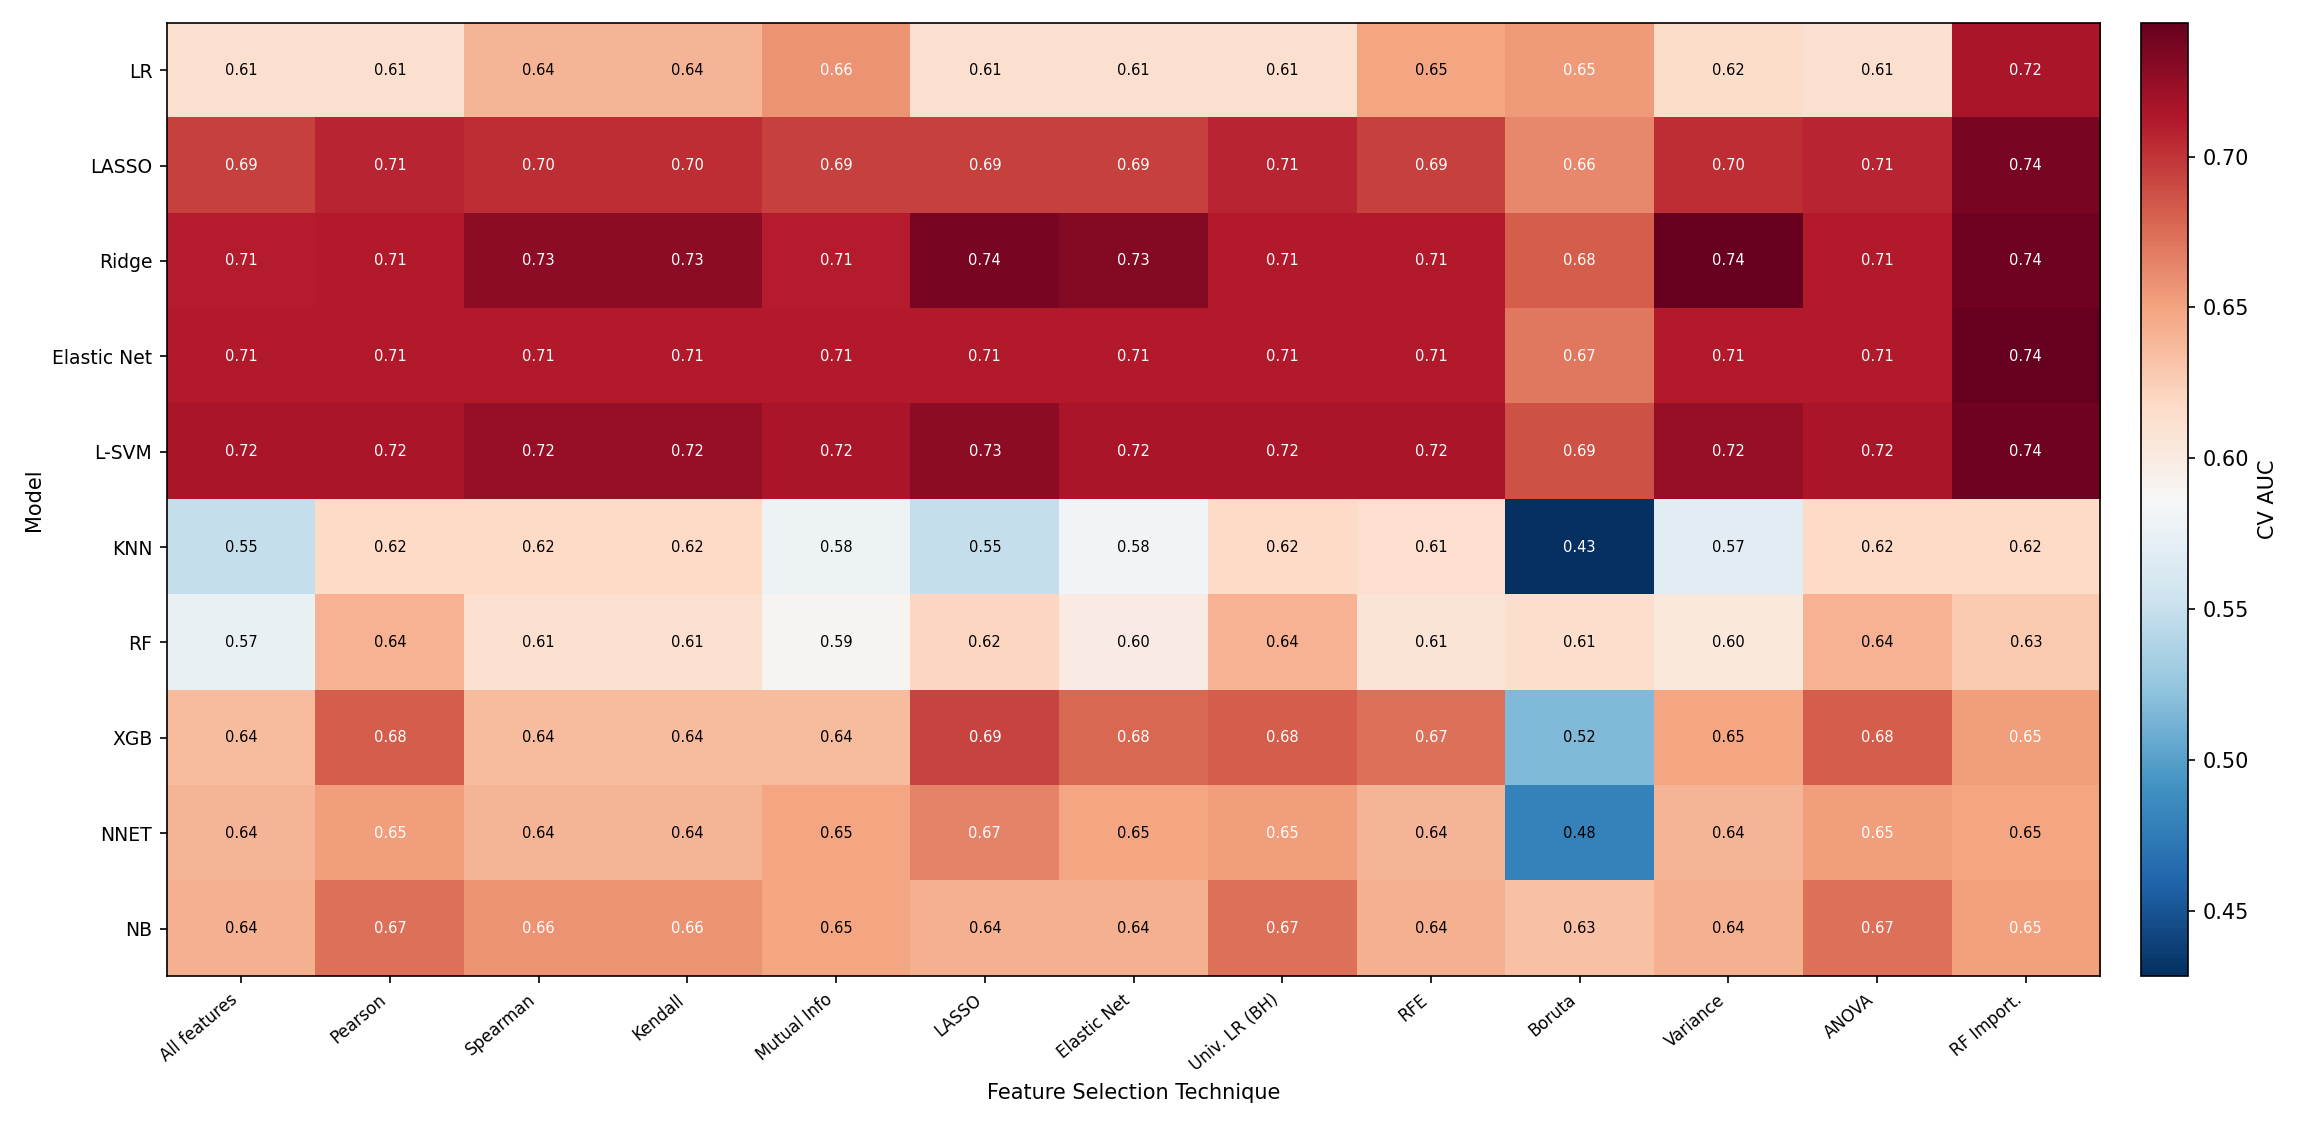
\includegraphics[width=\textwidth]{figures/heatmap_resection_cv_auc}
    \caption{Resection 3-fold CV AUC}
\end{subfigure}
\\[0.8em]
\begin{subfigure}[b]{\textwidth}
    \centering
    
\includegraphics[width=\textwidth]{figures/heatmap_soramic_auroc}
    \caption{Soramic transfer AUROC}
\end{subfigure}
\caption{Grid AUROC across the 10 classifiers ($y$-axis) $\times$ 13 feature-selection
techniques ($x$-axis) for the single best image embedding (raw, $\lambda=0.1$, slice-level
split): (a) resection 3-fold CV AUC, on which the best cell is selected, and (b) its transfer
to the Soramic ablation set.}
\label{fig:grid_heatmaps}
\end{figure}

\subsubsection*{Survival Analysis}

Table~\ref{tab:external_survival} summarises the Soramic stratification.
The high-risk group had significantly worse 2-year outcome than the low-risk group on both endpoints
(RFS $\tau=24$ log-rank $p=0.043$, HR $3.93$; TTR $\tau=24$ log-rank $p=0.024$, HR $7.26$).
The separation attenuated beyond 24 months (full-follow-up RFS log-rank $p=0.114$), consistent
with the 2-year focus established in Section~3.1. The low-risk group contained only 1--2 events,
which inflates the hazard-ratio confidence intervals, so the log-rank test is the more reliable read.

\begin{table}[H]
\centering
\small
\caption{Soramic survival stratification for the best downstream model
(frozen $k$-means cutoff, 90 high-risk / 10 low-risk). HR $>1$ indicates worse outcome in the
high-risk group.}
\label{tab:external_survival}
\begin{tabular}{llccc}
\hline
Endpoint & Horizon & Events (hi/lo) & HR (95\% CI) & Log-rank $p$ \\
\hline
RFS & $\tau=24$\,mo & 37 / 2 & 3.93 (0.94--16.38) & \textbf{0.043} \\
RFS & full         & 46 / 4 & 2.25 (0.80--6.32)  & 0.114 \\
TTR & $\tau=24$\,mo & 28 / 1 & 7.26 (0.98--54.01) & \textbf{0.024} \\
TTR & full         & 29 / 2 & 3.74 (0.88--15.96) & 0.056 \\
\hline
\end{tabular}
\end{table}

Figure~\ref{fig:km_rfs} shows the corresponding RFS Kaplan--Meier curves.

\begin{figure}[H]
\centering
\begin{subfigure}[b]{0.49\textwidth}
    \centering
    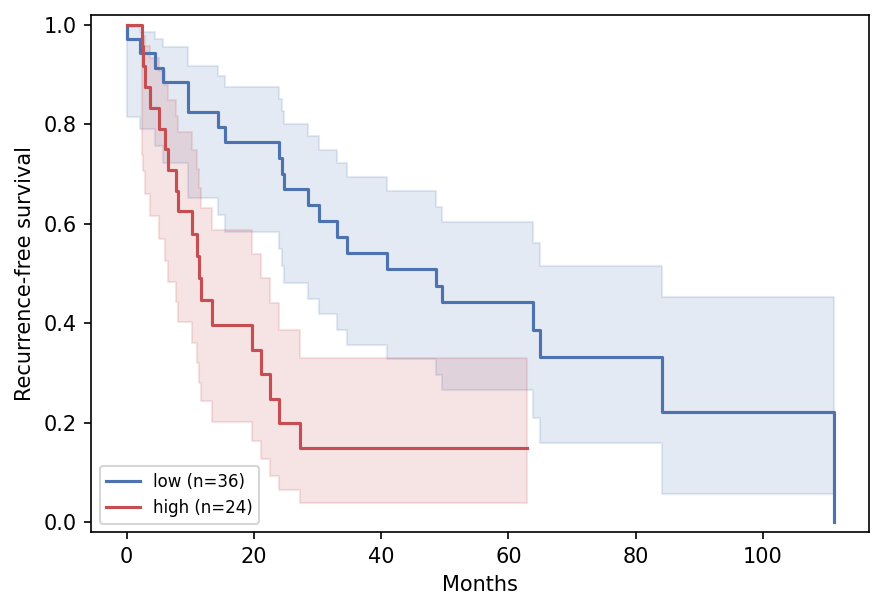
\includegraphics[width=\textwidth]{figures/km_rfs_resection}
    \caption{Resection}
\end{subfigure}
\hfill
\begin{subfigure}[b]{0.49\textwidth}
    \centering
    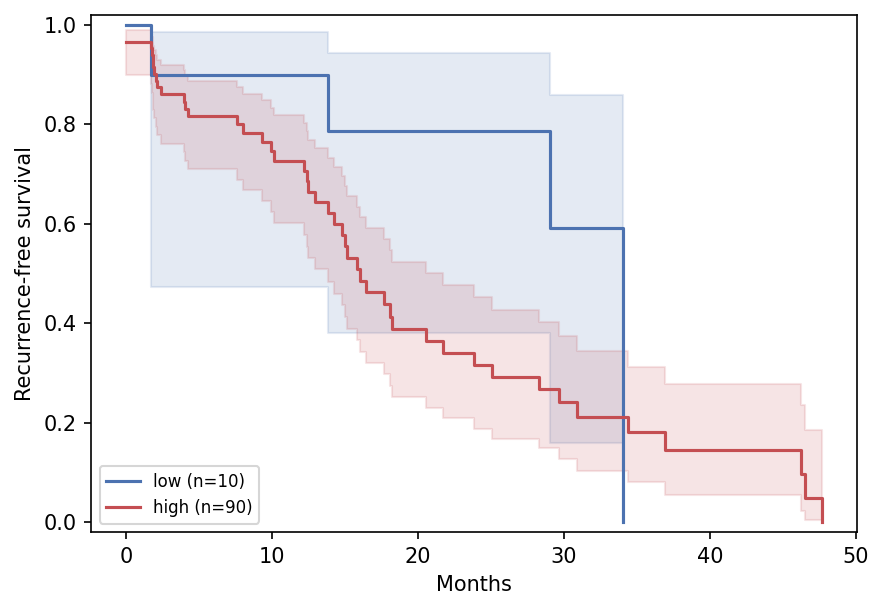
\includegraphics[width=\textwidth]{figures/km_rfs_soramic}
    \caption{Soramic}
\end{subfigure}
\caption{RFS Kaplan--Meier curves for the best downstream model, stratified by the resection
$k$-means cutoff into high- and low-risk groups. Shaded bands are 95\% confidence intervals.}
\label{fig:km_rfs}
\end{figure}


\section{Model Interpretability}
todo

\chapter{Conclusion}
todo



%%%%%%%%%%%%%%%%%%%%%%%%%%%%%%%%%%%%

\bibliographystyle{unsrt}
\renewcommand{\bibname}{References}
\addcontentsline{toc}{chapter}{References}
\bibliography{reference}

%%%%%%%%%%%%%%%%%%%%%%%%%%%%%%%%%%%%
\begin{appendices}

\chapter{RNA-seq Feature Selection Details}
\label{app:rna_fs}

The tables below list the 20 genes selected by DESeq2 from the full transcriptome
in the before-CV run (applied once to the complete task-filtered dataset),
along with their Benjamini--Hochberg adjusted $p$-values.
Genes passing BH correction at $p < 0.05$ are marked with an asterisk ($*$);
the remaining entries are fallback selections (top 20 by adjusted $p$-value).
For 1-year RFS, six genes pass BH correction; for 2-year RFS, three genes pass.
H19 in Table~\ref{tab:deseq_2y} is the sole gene intersecting the predefined HCC gene set.

\begin{table}[h]
\centering
\caption{DESeq2-selected genes for 1-year RFS prediction
(before-CV, full transcriptome, $n=56$).
Asterisk ($*$) denotes BH-adjusted $p < 0.05$.}
\label{tab:deseq_1y}
\begin{tabular}{lr}
\hline
Gene & BH-adjusted $p$-value \\
\hline
AL138889.1 & $5.84 \times 10^{-4}$\,* \\
AC135731.1 & $5.84 \times 10^{-4}$\,* \\
AC004889.1 & $3.33 \times 10^{-2}$\,* \\
CCDC26     & $3.93 \times 10^{-2}$\,* \\
INAFM2     & $4.67 \times 10^{-2}$\,* \\
AL160272.1 & $4.67 \times 10^{-2}$\,* \\
AC092068.2 & $5.43 \times 10^{-2}$ \\
LINC00514  & $5.46 \times 10^{-2}$ \\
AL031594.1 & $9.46 \times 10^{-2}$ \\
AL117328.2 & $1.07 \times 10^{-1}$ \\
AC005696.4 & $1.54 \times 10^{-1}$ \\
EGFL8      & $2.11 \times 10^{-1}$ \\
AC025580.2 & $2.11 \times 10^{-1}$ \\
AC006538.1 & $2.11 \times 10^{-1}$ \\
AC127070.4 & $2.53 \times 10^{-1}$ \\
AL353726.2 & $2.86 \times 10^{-1}$ \\
AC016355.1 & $3.32 \times 10^{-1}$ \\
AC008395.1 & $3.46 \times 10^{-1}$ \\
AL008638.3 & $3.46 \times 10^{-1}$ \\
AC102953.2 & $3.83 \times 10^{-1}$ \\
\hline
\end{tabular}
\end{table}

\begin{table}[h]
\centering
\caption{DESeq2-selected genes for 2-year RFS prediction
(before-CV, full transcriptome, $n=54$).
Asterisk ($*$) denotes BH-adjusted $p < 0.05$.
H19 (\textsuperscript{\dag}) is the sole intersection with the predefined HCC gene set.}
\label{tab:deseq_2y}
\begin{tabular}{lr}
\hline
Gene & BH-adjusted $p$-value \\
\hline
CAMK2N2    & $8.94 \times 10^{-3}$\,* \\
AC093826.2 & $3.18 \times 10^{-2}$\,* \\
LACC1      & $4.58 \times 10^{-2}$\,* \\
CSF2       & $1.77 \times 10^{-1}$ \\
HNRNPA1P9  & $1.77 \times 10^{-1}$ \\
AL445235.1 & $1.77 \times 10^{-1}$ \\
AC025580.2 & $1.77 \times 10^{-1}$ \\
AC025198.1 & $1.77 \times 10^{-1}$ \\
AC093525.8 & $1.77 \times 10^{-1}$ \\
OR52N5     & $1.97 \times 10^{-1}$ \\
RBMXL3     & $1.97 \times 10^{-1}$ \\
AC004241.5 & $1.97 \times 10^{-1}$ \\
AC138647.1 & $2.23 \times 10^{-1}$ \\
AL449283.1 & $2.73 \times 10^{-1}$ \\
AC130366.1 & $2.73 \times 10^{-1}$ \\
AC063947.2 & $4.55 \times 10^{-1}$ \\
H19\textsuperscript{\dag} & $4.63 \times 10^{-1}$ \\
SGSM1      & $4.63 \times 10^{-1}$ \\
HIGD2B     & $4.63 \times 10^{-1}$ \\
ZMYND12    & $4.63 \times 10^{-1}$ \\
\hline
\end{tabular}
\end{table}

%%%%%%%%%%%%%%%%%%%%%%%%%%%%%%%%%%%%

\chapter{Complete External Evaluation Metrics}
\label{app:external_metrics}

Tables~\ref{tab:soramic_metrics} and~\ref{tab:lausanne_metrics} provide full classification
metrics for all 16 contrastive models and the radiomic baseline on the Soramic ablation set
and the Lausanne cohort for 2-year RFS prediction.
Best head (LR or RF) per model is shown, ranked by AUROC.
``---'' denotes undefined NPV (all samples predicted positive).

\begin{table}[H]
\centering
\small
\caption{Soramic ablation set ($n=59$, 68\% positive): all models ranked by AUROC,
2-year RFS. Best head (LR or RF) per model shown.}
\label{tab:soramic_metrics}
\resizebox{\textwidth}{!}{%
\begin{tabular}{llrrrrrrr}
\hline
Head & Configuration & AUROC & AUPRC & Sens. & Spec. & PPV & NPV & F1 \\
\hline
LR & raw, $\lambda$=0.1, 2y\textsubscript{bCV} genes, $n$=10, patient & 0.732 & 0.865 & 0.846 & 0.389 & 0.750 & 0.538 & 0.795 \\
LR & raw, $\lambda$=0.1, frozen, $n$=all, slice                       & 0.718 & 0.838 & 0.846 & 0.389 & 0.750 & 0.538 & 0.795 \\
LR & raw, $\lambda$=0.0, frozen, $n$=all, patient                     & 0.702 & 0.840 & 0.897 & 0.222 & 0.714 & 0.500 & 0.795 \\
LR & raw, $\lambda$=0.0, frozen, $n$=all, slice                       & 0.684 & 0.804 & 0.974 & 0.278 & 0.745 & 0.833 & 0.844 \\
RF & raw, $\lambda$=0.1, predefined genes, $n$=10, slice              & 0.670 & 0.820 & 0.872 & 0.278 & 0.723 & 0.500 & 0.791 \\
LR & bbox, $\lambda$=0.1, unfrozen, $n$=10, slice                     & 0.669 & 0.791 & 1.000 & 0.000 & 0.667 & ---   & 0.800 \\
RF & raw, $\lambda$=0.1, frozen, $n$=all, patient                     & 0.635 & 0.819 & 1.000 & 0.000 & 0.684 & ---   & 0.812 \\
LR & raw, $\lambda$=0.1, unfrozen, $n$=10, slice                      & 0.615 & 0.816 & 0.385 & 0.778 & 0.789 & 0.368 & 0.517 \\
RF & raw, $\lambda$=0.0, unfrozen, $n$=10, slice                      & 0.606 & 0.734 & 1.000 & 0.000 & 0.684 & ---   & 0.812 \\
\hline
RF & \textit{Radiomic baseline}, 149 arterial features                 & 0.590 & 0.766 & 0.143 & 1.000 & 1.000 & 0.375 & 0.250 \\
\hline
RF & bbox, $\lambda$=0.1, frozen, $n$=all, slice                      & 0.577 & 0.719 & 0.972 & 0.000 & 0.660 & 0.000 & 0.787 \\
LR & raw, $\lambda$=0.1, predefined genes, $n$=10, patient            & 0.574 & 0.734 & 0.667 & 0.500 & 0.743 & 0.409 & 0.703 \\
LR & bbox, $\lambda$=0.1, unfrozen, $n$=10, patient                   & 0.539 & 0.710 & 0.944 & 0.056 & 0.667 & 0.333 & 0.782 \\
LR & bbox, $\lambda$=0.0, unfrozen, $n$=10, patient                   & 0.534 & 0.661 & 0.028 & 0.889 & 0.333 & 0.314 & 0.051 \\
RF & raw, $\lambda$=0.1, unfrozen, $n$=10, patient                    & 0.522 & 0.707 & 1.000 & 0.000 & 0.684 & ---   & 0.812 \\
\hline
LR & \textit{Radiomic baseline}, 149 arterial features                 & 0.518 & 0.671 & 0.657 & 0.389 & 0.676 & 0.368 & 0.667 \\
\hline
LR & bbox, $\lambda$=0.0, unfrozen, $n$=10, slice                     & 0.517 & 0.693 & 0.472 & 0.556 & 0.680 & 0.345 & 0.557 \\
RF & raw, $\lambda$=0.1, 2y\textsubscript{bCV} genes, $n$=10, slice   & 0.516 & 0.712 & 1.000 & 0.000 & 0.684 & ---   & 0.812 \\
LR & raw, $\lambda$=0.0, unfrozen, $n$=10, patient                    & 0.494 & 0.674 & 0.949 & 0.056 & 0.685 & 0.333 & 0.796 \\
\hline
\end{tabular}%
}
\end{table}

\begin{table}[H]
\centering
\small
\caption{Lausanne cohort ($n=66$, 74\% positive): all models ranked by AUROC,
2-year RFS. Best head (LR or RF) per model shown.}
\label{tab:lausanne_metrics}
\resizebox{\textwidth}{!}{%
\begin{tabular}{llrrrrrrr}
\hline
Head & Configuration & AUROC & AUPRC & Sens. & Spec. & PPV & NPV & F1 \\
\hline
RF & raw, $\lambda$=0.1, unfrozen, $n$=10, patient                    & 0.771 & 0.867 & 1.000 & 0.000 & 0.742 & ---   & 0.852 \\
RF & bbox, $\lambda$=0.1, frozen, $n$=all, slice                      & 0.614 & 0.810 & 0.979 & 0.059 & 0.746 & 0.500 & 0.847 \\
LR & raw, $\lambda$=0.1, 2y\textsubscript{bCV} genes, $n$=10, slice   & 0.655 & 0.850 & 1.000 & 0.000 & 0.742 & ---   & 0.852 \\
LR & raw, $\lambda$=0.0, unfrozen, $n$=10, patient                    & 0.618 & 0.827 & 0.980 & 0.059 & 0.750 & 0.500 & 0.850 \\
LR & raw, $\lambda$=0.0, unfrozen, $n$=10, slice                      & 0.600 & 0.844 & 0.980 & 0.059 & 0.750 & 0.500 & 0.850 \\
RF & bbox, $\lambda$=0.0, unfrozen, $n$=10, slice                     & 0.595 & 0.790 & 0.438 & 0.706 & 0.808 & 0.308 & 0.568 \\
LR & raw, $\lambda$=0.1, 2y\textsubscript{bCV} genes, $n$=10, patient & 0.563 & 0.806 & 0.694 & 0.353 & 0.756 & 0.286 & 0.723 \\
RF & raw, $\lambda$=0.0, frozen, $n$=all, slice                       & 0.556 & 0.803 & 0.959 & 0.059 & 0.746 & 0.333 & 0.839 \\
RF & bbox, $\lambda$=0.1, unfrozen, $n$=10, slice                     & 0.544 & 0.755 & 0.333 & 0.765 & 0.800 & 0.289 & 0.471 \\
\hline
LR & \textit{Radiomic baseline}, 149 arterial features                 & 0.531 & 0.748 & 0.422 & 0.625 & 0.760 & 0.278 & 0.543 \\
\hline
LR & raw, $\lambda$=0.1, frozen, $n$=all, patient                     & 0.534 & 0.775 & 0.939 & 0.118 & 0.754 & 0.400 & 0.836 \\
RF & bbox, $\lambda$=0.1, unfrozen, $n$=10, patient                   & 0.515 & 0.769 & 1.000 & 0.000 & 0.738 & ---   & 0.850 \\
LR & raw, $\lambda$=0.0, frozen, $n$=all, patient                     & 0.515 & 0.779 & 0.755 & 0.294 & 0.755 & 0.294 & 0.755 \\
\hline
RF & \textit{Radiomic baseline}, 149 arterial features                 & 0.506 & 0.747 & 0.067 & 0.875 & 0.600 & 0.250 & 0.120 \\
\hline
LR & raw, $\lambda$=0.1, unfrozen, $n$=10, slice                      & 0.497 & 0.753 & 0.204 & 0.765 & 0.714 & 0.250 & 0.317 \\
RF & bbox, $\lambda$=0.0, unfrozen, $n$=10, patient                   & 0.494 & 0.766 & 0.646 & 0.353 & 0.738 & 0.261 & 0.689 \\
RF & raw, $\lambda$=0.1, frozen, $n$=all, slice                       & 0.453 & 0.727 & 0.776 & 0.118 & 0.717 & 0.154 & 0.745 \\
RF & raw, $\lambda$=0.1, predefined genes, $n$=10, slice              & 0.477 & 0.755 & 0.796 & 0.176 & 0.736 & 0.231 & 0.765 \\
LR & raw, $\lambda$=0.1, predefined genes, $n$=10, patient            & 0.420 & 0.702 & 0.531 & 0.412 & 0.722 & 0.233 & 0.612 \\
\hline
\end{tabular}%
}
\end{table}

%%%%%%%%%%%%%%%%%%%%%%%%%%%%%%%%%%%%

\chapter{RNA-seq Baseline Full Results}
\label{app:rna_baseline_plots}

Three configurations were evaluated, all using DESeq2 feature selection
(BH-adjusted $p < 0.05$; fallback to top 20 genes by adjusted $p$-value),
3-fold stratified CV, $L_1$ logistic regression ($C \in \{0.001, 0.01, 0.1, 1\}$)
and random forest (depth $\in \{2, 4\}$, min leaf $\in \{5, 10, 15\}$):

\begin{description}
  \item[C1] \texttt{before\_cv}, full transcriptome (50,986 genes) — DESeq2 fit once on the
    full labelled dataset before CV (information leak; diagnostic only).
  \item[C2] \texttt{before\_cv}, predefined HCC gene set (2,146 genes) — same leakage
    setting but restricted to the curated HCC prior.
  \item[C3] \texttt{in\_cv}, predefined HCC gene set — statistically valid: DESeq2 refit
    inside each training fold.
\end{description}

\noindent Table~\ref{tab:rna_summary} summarises the best mean test AUROC per classifier.

\begin{table}[H]
\centering
\small
\caption{Best mean test AUROC per configuration and classifier for RNA-seq baselines.
C1 values are leakage-inflated (before-CV selection). C2 and C3 collapse to
majority-class prediction because no gene survives BH correction.}
\label{tab:rna_summary}
\begin{tabular}{lcccc}
\hline
Config & 1y LR & 1y RF & 2y LR & 2y RF \\
\hline
C1 — before-CV, all genes     & \textbf{0.686} & 0.601 & \textbf{0.864} & 0.761 \\
C2 — before-CV, predefined    & 0.500 & 0.570 & 0.500 & 0.505 \\
C3 — in-CV, predefined        & 0.500 & 0.500 & 0.500 & 0.508 \\
\hline
\end{tabular}
\end{table}

\section*{C1 --- Before-CV, Full Transcriptome}

\begin{figure}[H]
\centering
\begin{subfigure}[b]{0.48\textwidth}
    \centering
    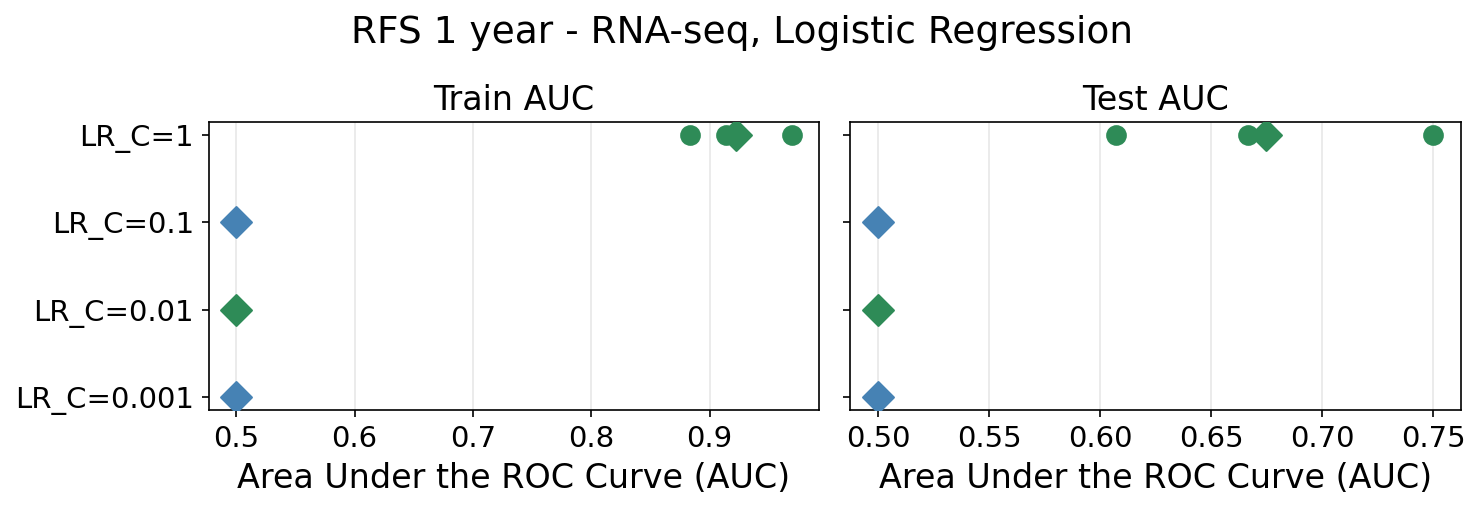
\includegraphics[width=\textwidth]{figures/baseline_c1_1y_lr}
    \caption{1-year RFS, LR}
\end{subfigure}
\hfill
\begin{subfigure}[b]{0.48\textwidth}
    \centering
    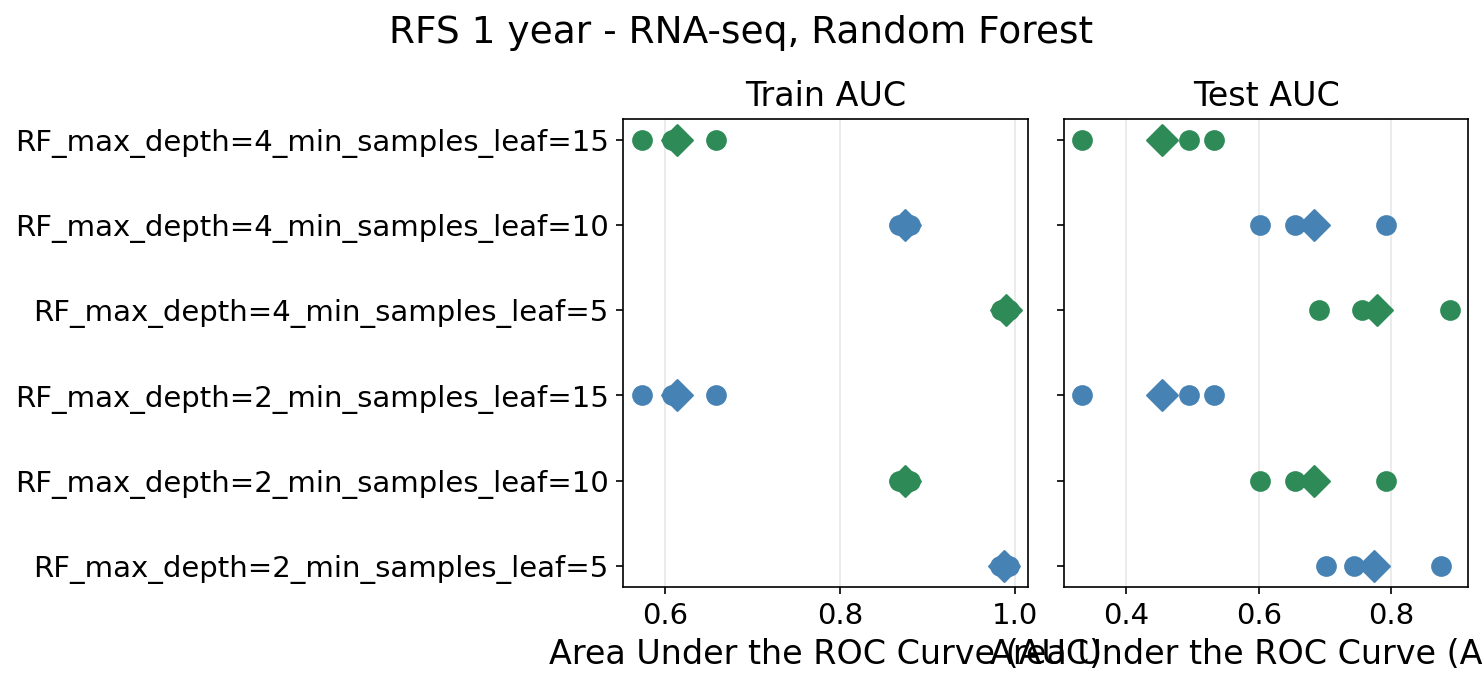
\includegraphics[width=\textwidth]{figures/baseline_c1_1y_rf}
    \caption{1-year RFS, RF}
\end{subfigure}
\\[0.6em]
\begin{subfigure}[b]{0.48\textwidth}
    \centering
    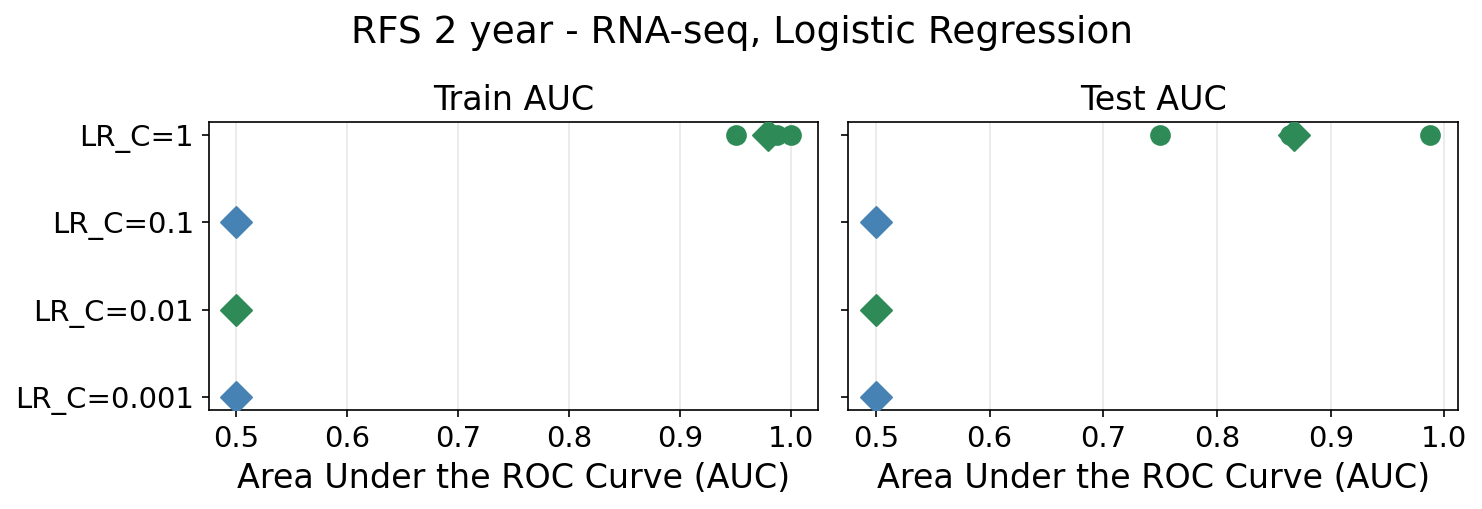
\includegraphics[width=\textwidth]{figures/baseline_c1_2y_lr}
    \caption{2-year RFS, LR}
\end{subfigure}
\hfill
\begin{subfigure}[b]{0.48\textwidth}
    \centering
    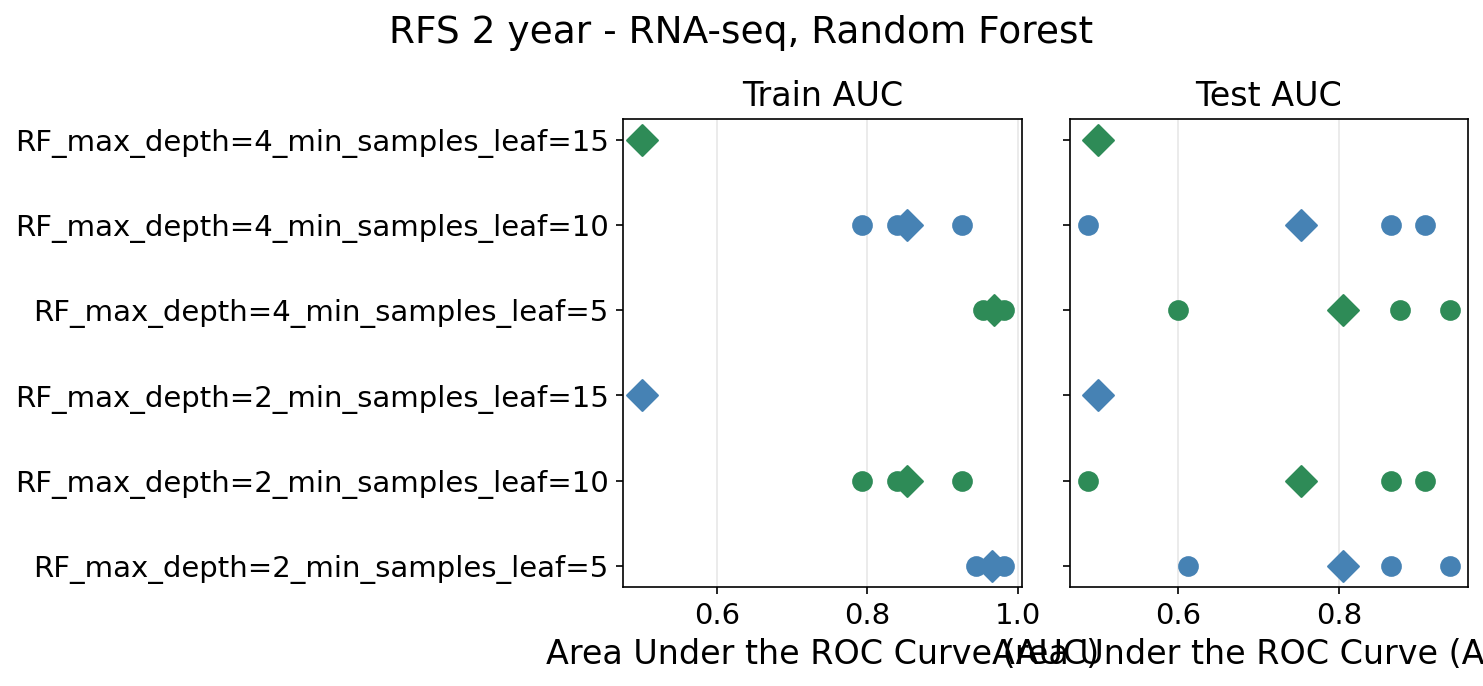
\includegraphics[width=\textwidth]{figures/baseline_c1_2y_rf}
    \caption{2-year RFS, RF}
\end{subfigure}
\caption{C1 (before-CV, full transcriptome): 3-fold CV AUROC strip plots.
Circles = per-fold AUC; diamonds = mean. Values are leakage-inflated.}
\label{fig:baseline_c1}
\end{figure}

\section*{C2 --- Before-CV, Predefined HCC Genes}

\begin{figure}[H]
\centering
\begin{subfigure}[b]{0.48\textwidth}
    \centering
    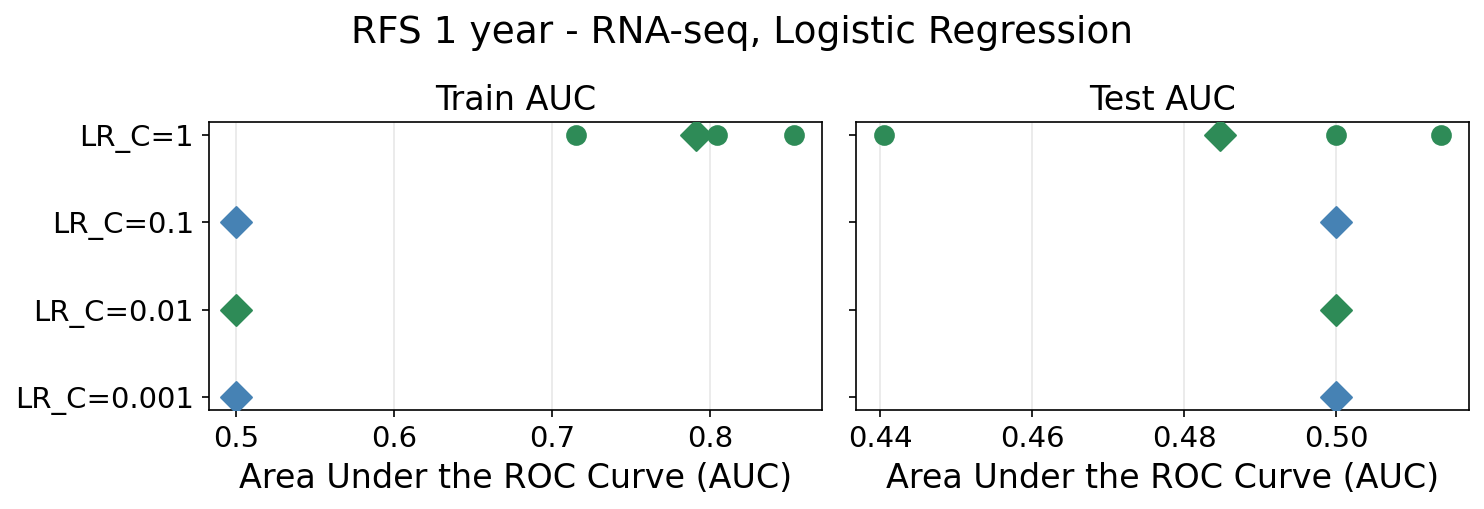
\includegraphics[width=\textwidth]{figures/baseline_c2_1y_lr}
    \caption{1-year RFS, LR}
\end{subfigure}
\hfill
\begin{subfigure}[b]{0.48\textwidth}
    \centering
    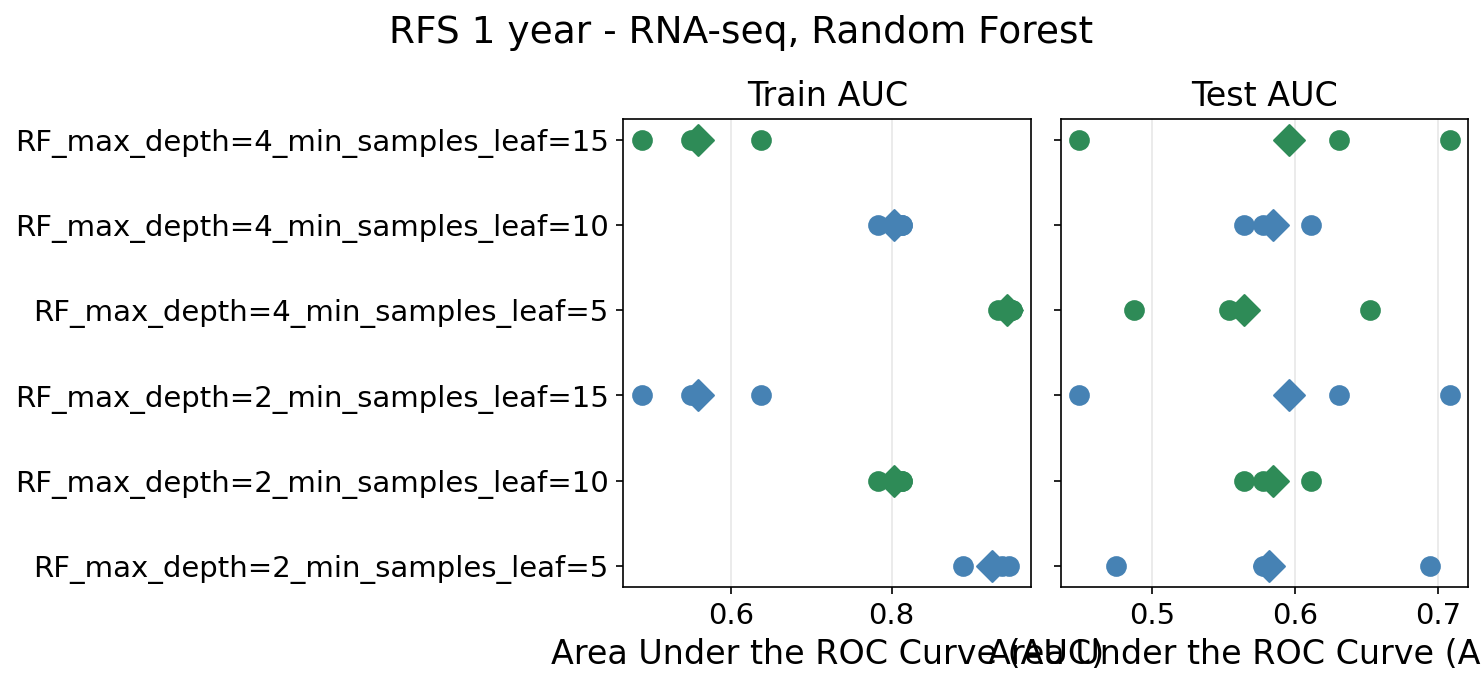
\includegraphics[width=\textwidth]{figures/baseline_c2_1y_rf}
    \caption{1-year RFS, RF}
\end{subfigure}
\\[0.6em]
\begin{subfigure}[b]{0.48\textwidth}
    \centering
    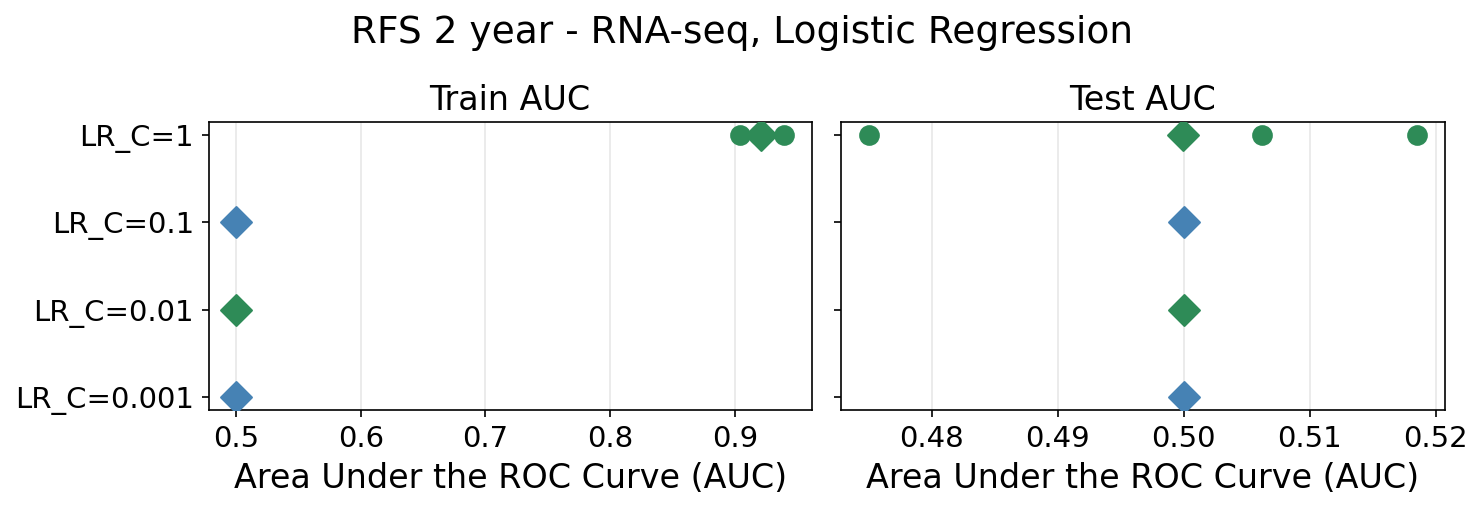
\includegraphics[width=\textwidth]{figures/baseline_c2_2y_lr}
    \caption{2-year RFS, LR}
\end{subfigure}
\hfill
\begin{subfigure}[b]{0.48\textwidth}
    \centering
    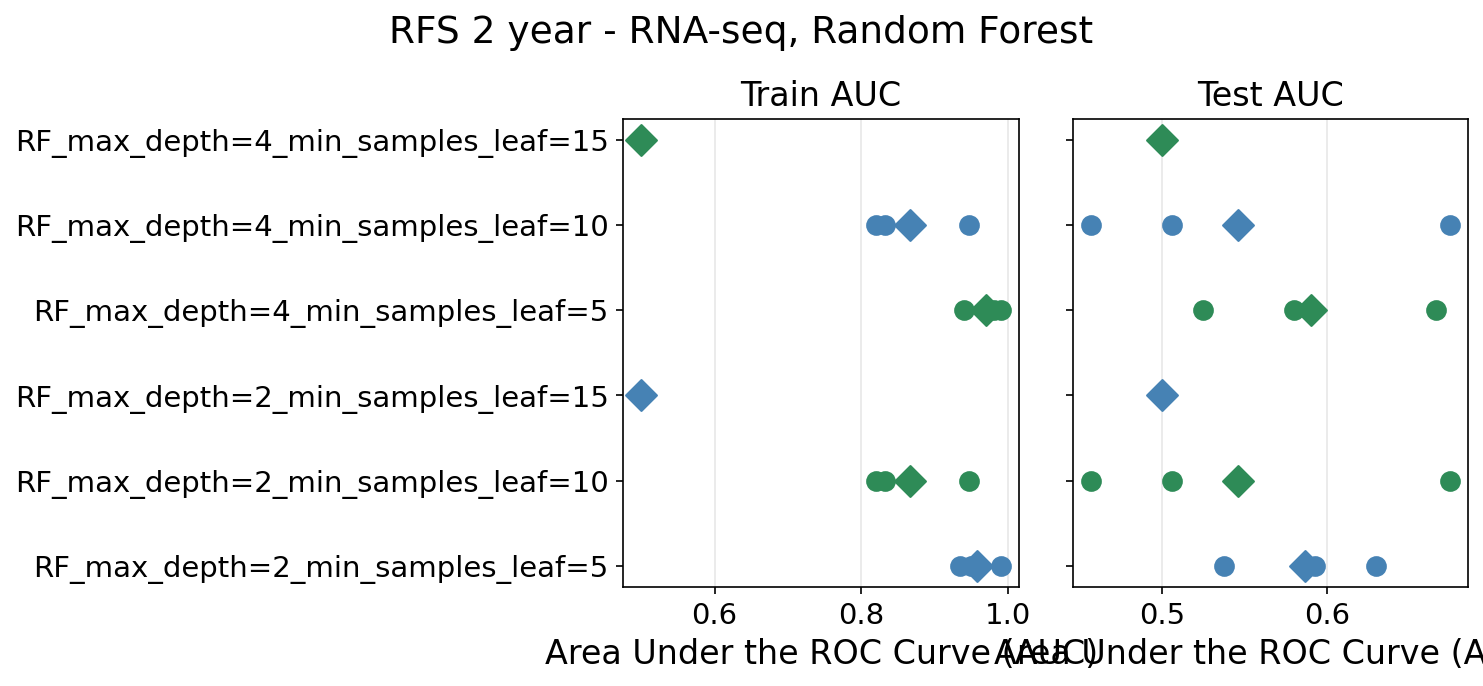
\includegraphics[width=\textwidth]{figures/baseline_c2_2y_rf}
    \caption{2-year RFS, RF}
\end{subfigure}
\caption{C2 (before-CV, predefined HCC genes): all models collapse to near-chance AUROC because
no gene survives BH correction; every fold uses the top-20 fallback.}
\label{fig:baseline_c2}
\end{figure}

\section*{C3 --- In-CV, Predefined HCC Genes}

\begin{figure}[H]
\centering
\begin{subfigure}[b]{0.48\textwidth}
    \centering
    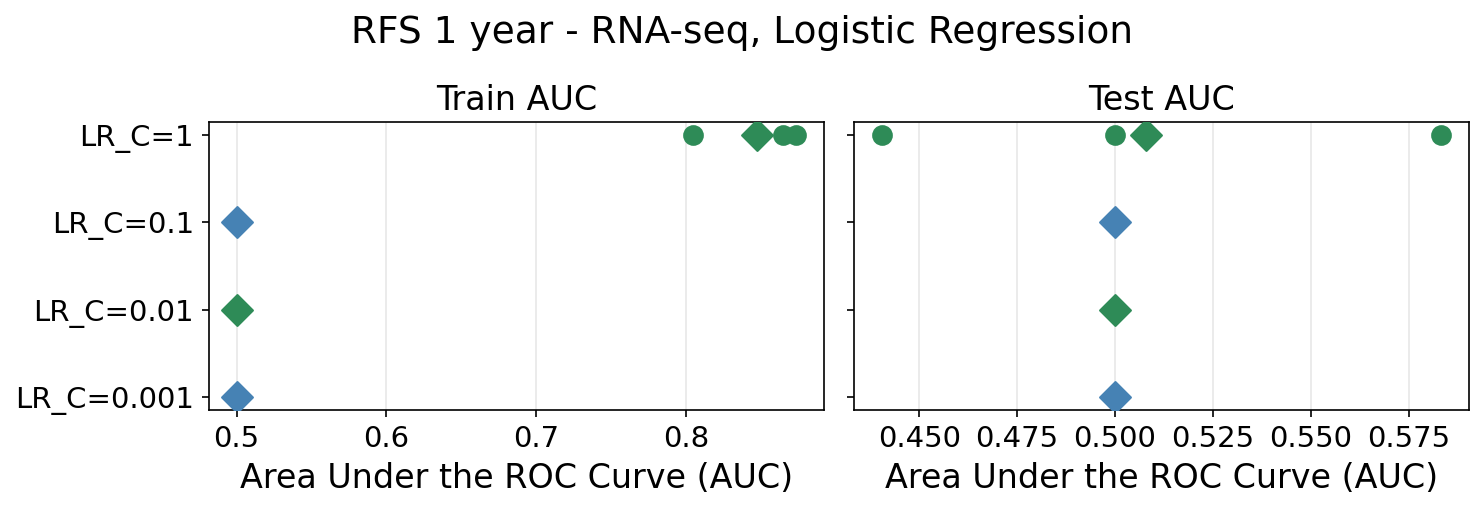
\includegraphics[width=\textwidth]{figures/baseline_c3_1y_lr}
    \caption{1-year RFS, LR}
\end{subfigure}
\hfill
\begin{subfigure}[b]{0.48\textwidth}
    \centering
    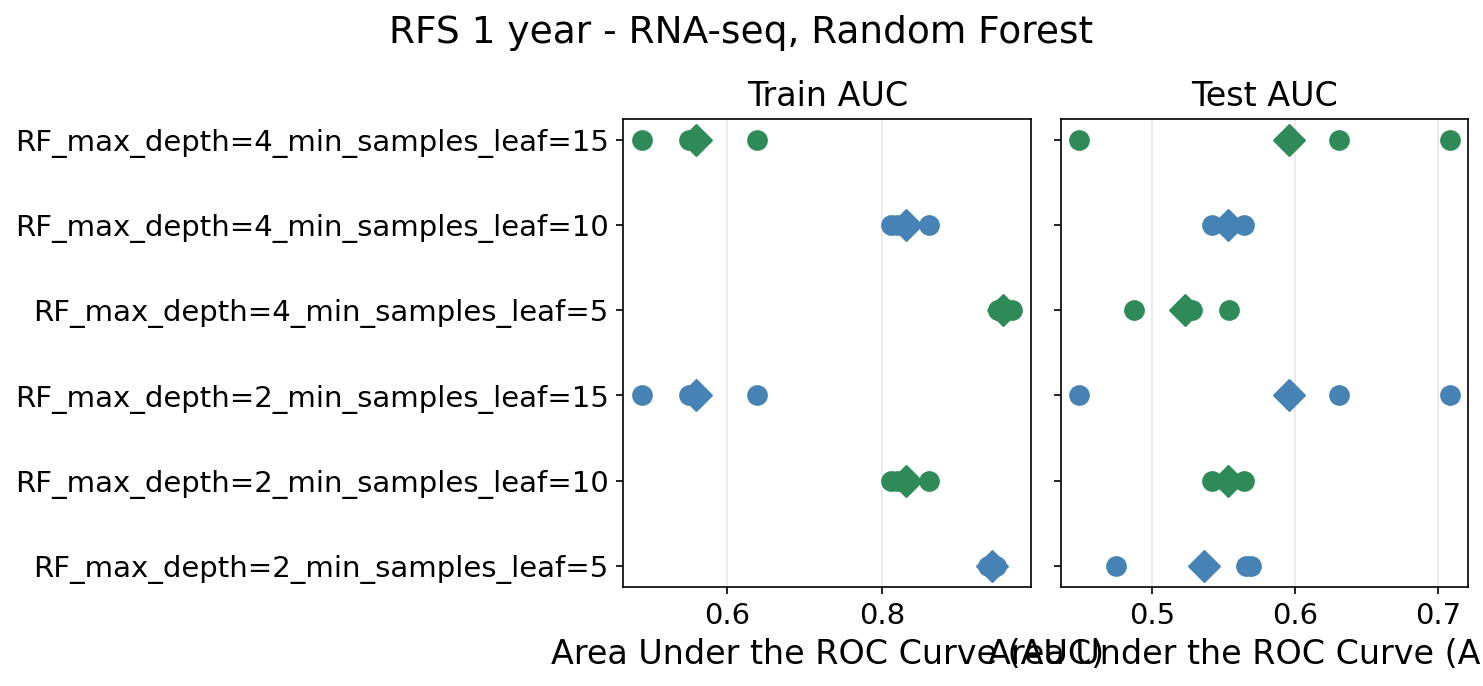
\includegraphics[width=\textwidth]{figures/baseline_c3_1y_rf}
    \caption{1-year RFS, RF}
\end{subfigure}
\\[0.6em]
\begin{subfigure}[b]{0.48\textwidth}
    \centering
    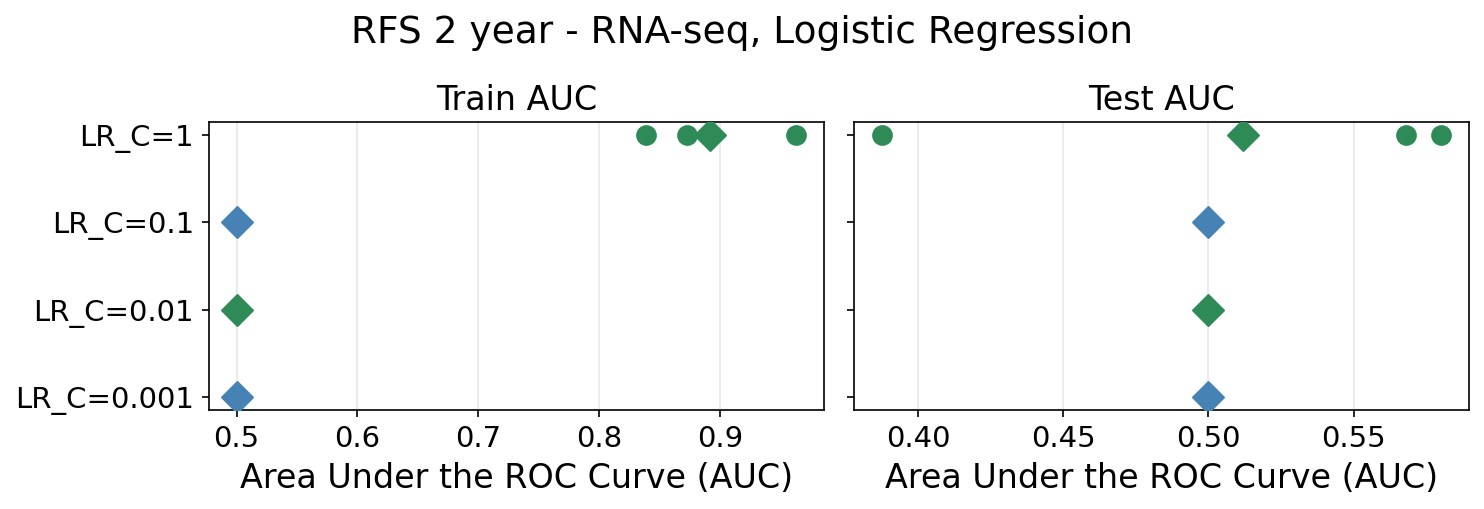
\includegraphics[width=\textwidth]{figures/baseline_c3_2y_lr}
    \caption{2-year RFS, LR}
\end{subfigure}
\hfill
\begin{subfigure}[b]{0.48\textwidth}
    \centering
    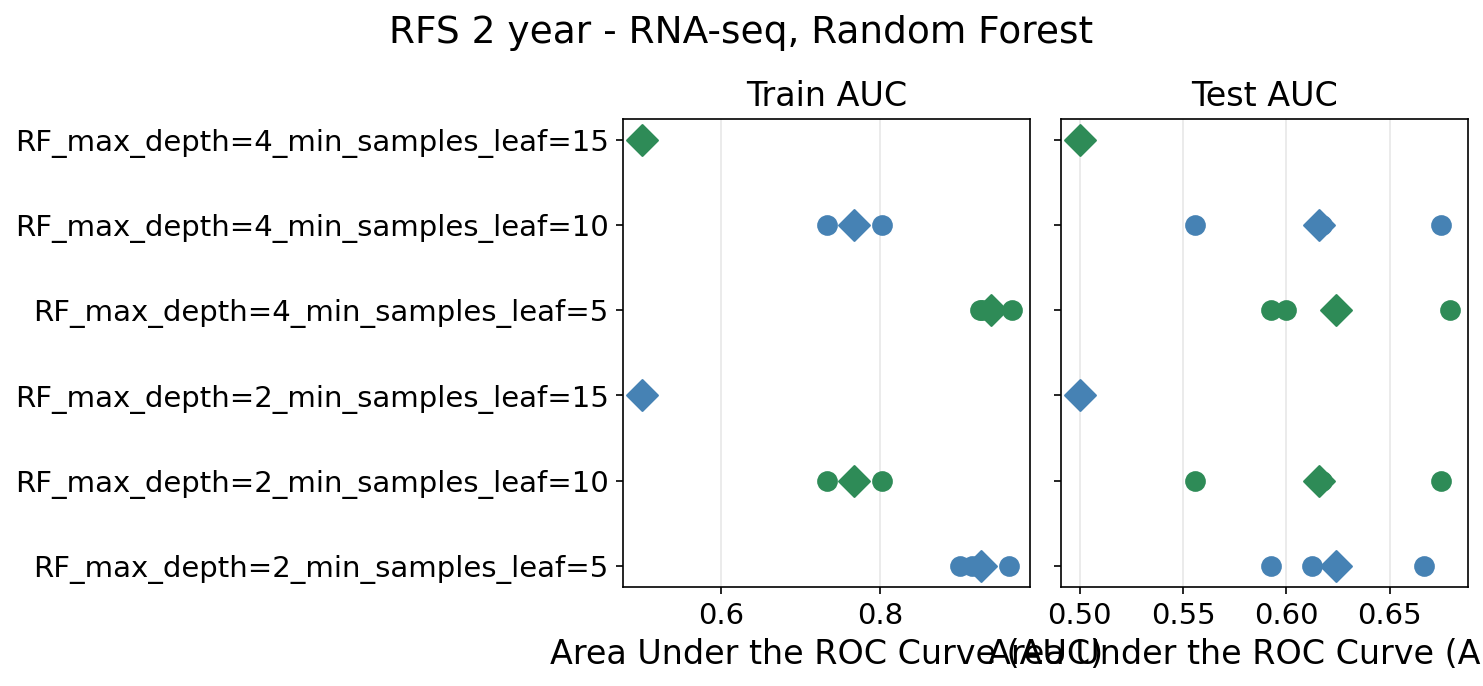
\includegraphics[width=\textwidth]{figures/baseline_c3_2y_rf}
    \caption{2-year RFS, RF}
\end{subfigure}
\caption{C3 (in-CV, predefined HCC genes): the statistically valid configuration.
Performance matches C2, confirming the predefined gene set carries no detectable
differential expression signal at this cohort size.}
\label{fig:baseline_c3}
\end{figure}


\end{appendices}

\end{document}
